%! suppress = EscapeHashOutsideCommand
%! suppress = Quote
%! suppress = MissingImport
%! suppress = MissingLabel
%! suppress = LineBreak

% CLI args https://tex.stackexchange.com/a/1501
\newif\ifhandout
\input{flags}

%! suppress = MissingLabel
%! suppress = DocumentclassNotInRoot
%! suppress = DiscouragedUseOfDef

% * Make friends tikz & colors
%   https://en.wikibooks.org/wiki/LaTeX/Colors
% * To enable vertical top alignment globally
%   https://tex.stackexchange.com/questions/9889/positioning-content-at-the-top-of-a-beamer-slide-by-default
% * Set handout from CLI
%   https://tex.stackexchange.com/a/1501
\ifhandout
\documentclass[usenames, dvipsnames, handout]{beamer} % https://tex.stackexchange.com/questions/224091/beamer-how-to-disable-pause-temporarily
\else
\documentclass[usenames, dvipsnames]{beamer}
\fi
% ------------------------------------------------

% Graphics
\usepackage{color}
\usepackage{tabularx}
\usepackage{tikz}
% https://tikz.dev/tikz-graphs
\usetikzlibrary{positioning, shapes.geometric, arrows, automata, graphs}
\tikzset{
    expr/.style={ellipse, draw=gray!60, fill=gray!5, very thick, minimum size=7mm, yshift=0.7cm},
    hexpr/.style={ellipse, draw=gray!60, fill=blue!15, very thick, minimum size=7mm, yshift=0.7cm},
    stmt/.style={rectangle, draw=gray!60, fill=gray!5, very thick, minimum size=5mm, yshift=0.7cm},
    decl/.style={rectangle, draw=blue!60, fill=gray!5, very thick, minimum size=5mm, yshift=0.7cm},
    hdecl/.style={rectangle, draw=blue!60, fill=blue!15, very thick, minimum size=5mm, yshift=0.7cm},
    subtree/.style={shape border rotate=90, isosceles triangle, draw=gray!60, fill=gray!5, very thick, minimum size=5mm, yshift=0.0cm},
}
\usepackage{blkarray}
\usepackage{graphicx}
\usepackage{forest} % https://tex.stackexchange.com/questions/198405/how-to-change-the-color-of-subtrees-in-tikz-qtree
% ------------------------------------------------

% Math
\usepackage{amsmath, amsfonts}
\usepackage{amssymb}
\usepackage{proof}
\usepackage{mathrsfs}
% Crossed-out symbols
% https://tex.stackexchange.com/questions/75525/how-to-write-crossed-out-math-in-latex
\usepackage[makeroom]{cancel}
\usepackage{mathtools}
% ------------------------------------------------

% Additional font sizes
% https://www.overleaf.com/learn/latex/Questions/How_do_I_adjust_the_font_size%3F
\usepackage{moresize}
% Additional colors
% https://www.overleaf.com/learn/latex/Using_colours_in_LaTeX
\usepackage{xcolor}
% Textual math symbols
\usepackage{textcomp}
% ------------------------------------------------

% Language
\usepackage[utf8] {inputenc}
\usepackage[T2A] {fontenc}
\usepackage[english, russian] {babel}
\usepackage{indentfirst, verbatim}
\usetikzlibrary{cd, babel}
% ------------------------------------------------

% Fonts: https://sites.math.washington.edu/~reu/docs/latex_symbols.pdf
\usepackage{stmaryrd}
\usepackage{cmbright}
\usepackage{wasysym}
\usepackage[weather]{ifsym} % https://tex.stackexchange.com/questions/100424/how-to-use-the-ifsym-package
% https://tex.stackexchange.com/questions/615300/pdflatex-builtin-glyph-names-is-empty
\pdfmapline{=dictsym DictSym <dictsym.pfb}
\pdfmapline{=pigpen <pigpen.pfa}
\usepackage{dictsym}
% ------------------------------------------------

% Code
% * Needs -shell-escape build flag
%   https://tex.stackexchange.com/questions/99475/how-to-invoke-latex-with-the-shell-escape-flag-in-texstudio-former-texmakerx
% * Set build directory
%   https://tex.stackexchange.com/questions/339931/latex-minted-package-using-custom-output-directory-build
\usepackage{minted}
\setminted{xleftmargin=\parindent, autogobble, escapeinside=\#\#}
% ------------------------------------------------

% Template
\usetheme{CambridgeUS}
\usecolortheme{dolphin}
% https://tex.stackexchange.com/questions/231439/beamer-how-to-make-font-larger-for-page-numbers
\setbeamerfont{headline}{size=\scriptsize}
\setbeamerfont{footline}{size=\scriptsize}
% Remove heddline
% https://tex.stackexchange.com/questions/33146/how-could-i-remove-a-header-in-a-beamer-presentation
%\setbeamertemplate{headline}{}
% Slide sizes
% https://tex.stackexchange.com/questions/56768/how-to-set-a-small-default-font-size-with-beamer
%\geometry{paperwidth=140mm,paperheight=105mm} % 4:3
\geometry{paperwidth=168mm,paperheight=105mm} % 16:10
% Remove navigation bar
% https://stackoverflow.com/questions/3210205/how-to-get-rid-of-navigation-bars-in-beamer
\beamertemplatenavigationsymbolsempty
% ------------------------------------------------

% Bullets
% https://9to5science.com/change-bullet-style-formatting-in-beamer
% https://tex.stackexchange.com/questions/185742/i-need-to-change-color-of-beamer-itemize-and-subitem-separately
\setbeamertemplate{itemize item}{\scriptsize\raise1.25pt\hbox{\donotcoloroutermaths$\blacktriangleright$}}
\setbeamertemplate{itemize subitem}{\scriptsize\raise1.5pt\hbox{\donotcoloroutermaths$\blacktriangleright$}}
\setbeamertemplate{itemize subsubitem}{\tiny\raise1.5pt\hbox{\donotcoloroutermaths$\blacktriangleright$}}
\setbeamertemplate{enumerate item}{\insertenumlabel.}
\setbeamertemplate{enumerate subitem}{\insertenumlabel.\insertsubenumlabel}
\setbeamertemplate{enumerate subsubitem}{\insertenumlabel.\insertsubenumlabel.\insertsubsubenumlabel}
% ------------------------------------------------

% Table of contents format
% https://tex.stackexchange.com/questions/642927/format-table-of-contents-in-beamer
\setbeamertemplate{section in toc}{%
        {\color{blue}\inserttocsectionnumber.}
    \inserttocsection\par%
}
\setbeamertemplate{subsection in toc}{%
        {\color{blue}\hspace{1em}\scriptsize\raise1.25pt\hbox{\donotcoloroutermaths$\blacktriangleright$}}
    \inserttocsubsection\par%
}
\setbeamertemplate{subsubsection in toc}{%
        {\color{blue}\hspace{2em}\tiny\raise1.25pt\hbox{\donotcoloroutermaths$\blacktriangleright$}}
    \inserttocsubsubsection\par%
}
% ------------------------------------------------

% Misc
\usepackage{multicol}
\usepackage{hyperref}
\usepackage{soul} % https://tex.stackexchange.com/questions/23711/strikethrough-text
% ------------------------------------------------

% Fix \pause for amsmath package envs (black black magic)
% https://tex.stackexchange.com/questions/16186/equation-numbering-problems-in-amsmath-environments-with-pause/75550#75550
% https://tex.stackexchange.com/questions/6348/problem-with-beamers-pause-in-alignments
%! suppress = Makeatletter
\makeatletter
\let\save@measuring@true\measuring@true
\def\measuring@true{%
    \save@measuring@true
    \def\beamer@sortzero##1{\beamer@ifnextcharospec{\beamer@sortzeroread{##1}}{}}%
    \def\beamer@sortzeroread##1<##2>{}%
    \def\beamer@finalnospec{}%
}
%! suppress = Makeatletter
\makeatother
% ------------------------------------------------

% Sections
\newcommand{\sectionplan}[1]{\section{#1}%
    \begin{frame}[noframenumbering]{Содержание}
        \tableofcontents[currentsection]
    \end{frame}
}
\newcommand{\subsectionplan}[1]{\subsection{#1}%
    \begin{frame}[noframenumbering]{Содержание}
        \tableofcontents[currentsubsection]
    \end{frame}
}
% ------------------------------------------------

% Footnotes
\renewcommand{\thefootnote}{\arabic{footnote}}
\renewcommand{\thempfootnote}{\arabic{mpfootnote}}
% https://tex.stackexchange.com/questions/28465/multiple-footnotes-at-one-point
\usepackage{fnpct}
% ------------------------------------------------

% Links
% Colors also links on slide foot.
%\hypersetup{
%    colorlinks=true,
%    citecolor=blue,
%    linkcolor=blue,
%    urlcolor=blue
%}
% ------------------------------------------------

% Appendix
% Slide numbers
% https://tex.stackexchange.com/questions/70448/dont-count-backup-slides
\usepackage{appendixnumberbeamer}
\newcommand{\backupbegin}{
    \newcounter{framenumbervorappendix}
    \setcounter{framenumbervorappendix}{\value{framenumber}}
}
\newcommand{\backupend}{
    \addtocounter{framenumbervorappendix}{-\value{framenumber}}
    \addtocounter{framenumber}{\value{framenumbervorappendix}}
}
% ------------------------------------------------

% Custom commands
% * Decor
\newcommand{\newtopic}[0]{$+$} % item: new topic on "in previous series"
\newcommand{\then}{$\Rightarrow$} % item: consequences
\newcommand{\pop}[0]{\SunCloud} %item:  general eduation
\newcommand{\popslide}[0]{(\pop)}
\newcommand{\advanced}[0]{$\varhexstar$} % item: advanced science
\newcommand{\advancedslide}[0]{(\advanced)}
\newcommand{\practical}[0]{\dstechnical} % item: practical programming notions
\newcommand{\practicalslide}[0]{(\practical)}
\newcommand{\todo}[0]{todo} % item: question
\newcommand{\answer}[0]{\Lightning} % item: answer to the previous question
\newcommand{\eg}[0]{e.g.} % item: example
\newcommand{\defi}[0]{$\Delta$} % item: definition on smth
\newcommand{\textdefi}[1]{\textbf{#1}}
\newcommand{\positive}{$+$} % item: pros
\newcommand{\negative}{{\color{red} $-$}} % item: cons
\newcommand%! suppress = EscapeHashOutsideCommand
\NB[1][0.3]{N\kern-#1em{B}} % default kern amount: -0.3em
\renewcommand{\emph}[1]{{\color{blue} \textit{#1}}}
\newcommand{\vocab}[1]{\textbf{#1}} % item: important new word
% * Lambda calculi
\newcommand{\comb}[1]{\mathbf{#1}} % defined combinator
\newcommand{\term}[1]{\mathbf{#1}} % predefined lambda-term reference
\newcommand{\termdef}{\coloneqq} % lamda term binding
\newcommand{\step}{\rightsquigarrow} % reduction step
\newcommand{\sstep}{\twoheadrightarrow} % multiple steps reduction
\newcommand{\ap}{~} % lambda-term application
\newcommand{\subst}[3]{\left[#2 \mapsto #3 \right] #1} % substitution
\newcommand{\eqbeta}{=_\beta} % beta equality
\newcommand{\eqeta}{=_\eta} % eta-equality
\newcommand{\eqt}{=} % tree-equality of terms
\newcommand{\tlist}[1]{\term{[}#1\term{]}} % list-term
% * Legacy
%\newcommand{\err}[0]{\textcolor{red}{ошибка}} % compilation error

% ------------------------------------------------

% Speaker notes
% https://tex.stackexchange.com/questions/114219/add-notes-to-latex-beamer
% https://tex.stackexchange.com/questions/35444/split-beamer-notes-across-multiple-notes-pages/35496#35496
%\setbeameroption{show notes on second screen=right} % enable speaker notes
%--------------------------------------

\author[]{Андрей Стоян, Илья Колегов, Дмитрий Халанский}
\institute[MSE ITMO]{MSE ITMO}


\title[11. Стандартные монады]{Практика 11. Стандартные монады}
\date{осень 2024}

\begin{document}

    \setcounter{framenumber}{-1}
    \maketitle

    \begin{frame}[fragile]{В предыдущих сериях}
        \begin{itemize}
            \item Классы типов \mintinline{haskell}|Functor|, \mintinline{haskell}|Applicative| и \mintinline{haskell}|Monad|
            \item Стандартные монады \mintinline{haskell}|Identity|, \mintinline{haskell}|Maybe| и \mintinline{haskell}|[]|
            \item[\newtopic] Стандартные монады \mintinline{haskell}|Reader|, \mintinline{haskell}|Writer|, \mintinline{haskell}|State|, \mintinline{haskell}|IO|, \mintinline{haskell}|Except|
        \end{itemize}
    \end{frame}

    \begin{frame}[noframenumbering]{Содержание}
        \tableofcontents
    \end{frame}


    \sectionplan{Монада Writer}

    \begin{frame}[fragile]{Монада \mintinline{haskell}|Writer|}
        \begin{minted}{haskell}
            newtype Writer w a = Writer { runWriter :: (w, a) }
        \end{minted}
        \begin{itemize}
            \item[\todo] Реализуйте \mintinline{haskell}|Functor| для \mintinline{haskell}|Writer|
            \item[\todo] Реализуйте \mintinline{haskell}|Applicative| для \mintinline{haskell}|Writer|
            \item[\todo] Реализуйте \mintinline{haskell}|Monad| для \mintinline{haskell}|Writer|
            \item[\todo] Реализуйте следующий код с помощью монады \mintinline{haskell}|Writer|
        \end{itemize}
        \vspace{-1em}
        \begin{columns}[onlytextwidth]
            \begin{column}[t]{0.485\textwidth}
                \begin{minted}{haskell}
                    f a b =
                      let (w1, x) = g a in
                      let w2 = w1 <> "ou" in
                      let (w3, y) = h b in
                      (w2 <> w3, x + y)
                \end{minted}
            \end{column}\hfill%
            \begin{column}[t]{0.485\textwidth}
                \pause
                \begin{minted}{haskell}
                    f a b = runWriter do
                      x <- g a
                      tell "ou"
                      y <- h b
                      pure (x + y)

                    tell :: w -> Writer w ()
                    tell w = Writer (w, ())
                \end{minted}
            \end{column}
        \end{columns}
    \end{frame}


    \sectionplan{Монада Reader}

    \begin{frame}[fragile]{Монада \mintinline{haskell}|Reader|}
        \begin{minted}{haskell}
            newtype Reader e a = Reader { runReader e -> a }
        \end{minted}
        \begin{itemize}
            \item[\todo] Реализуйте \mintinline{haskell}|Functor| для \mintinline{haskell}|Reader|
            \item[\todo] Реализуйте \mintinline{haskell}|Applicative| для \mintinline{haskell}|Reader|
            \item[\todo] Реализуйте \mintinline{haskell}|Monad| для \mintinline{haskell}|Reader|
            \item[\todo] Реализуйте следующий код с помощью монады \mintinline{haskell}|Reader|
        \end{itemize}
        \vspace{-1em}
        \begin{columns}[onlytextwidth]
            \begin{column}[t]{0.485\textwidth}
                \begin{minted}{haskell}
                    f :: Int -> Env -> Int
                    f a env =
                      let x = g a env in
                      let y = intField env in
                      let z = h env in
                      x + y + z
                \end{minted}
            \end{column}\hfill%
            \begin{column}[t]{0.485\textwidth}
                \pause
                \begin{minted}{haskell}
                    f :: Int -> Env -> Int
                    f a = runReader do
                      x <- g a
                      y <- asks intField
                      z <- h
                      pure (x + y + z)

                    asks :: (e -> e') -> Reader e e'
                    asks = Reader
                \end{minted}
            \end{column}
        \end{columns}
    \end{frame}

    \begin{frame}[fragile]{Мотивация \mintinline{haskell}|Reader|}
        \vspace{-0.5em}
        \begin{itemize}
            \item[\eg] Конфигурация программы, нужна большому количеству кода
            \item[\eg] По некоторой функциональности нужно абстрагироваться
            \begin{itemize}
                \item Возможности подмены реализации,
                \item[\eg] Для тестирования
            \end{itemize}
            \item Вариант: singleton object --- глобальный объект, который доступен отовсюду
            \begin{itemize}
                \item[\positive] В тупом варианте очень просто и везде работает (почти)
                \item[\negative] Тяжело подменить --- минус тестируемость
                \item[\negative] Нет гранулярного контроля доступа к глобальному объекту
            \end{itemize}
            \item Вариант: передача везде доп. аргумента --- окружения (коробочка со значениями и функциями)
            \begin{itemize}
                \item[\positive] Зависимость записана в сигнатурах
                \item[\positive] Просто и работает
                \item[\negative] Передача всегда доп. аргумента засоряет код
                \item[\then] Нужен механизм неявной передачи некоторых аргументов\footnote{Можно переиспользовать передачу словарей классов типов: \href{https://ghc.gitlab.haskell.org/ghc/doc/users_guide/exts/implicit_parameters.html}{\color{blue} ImplicitParams}.}
            \end{itemize}
        \end{itemize}
    \end{frame}

    \begin{frame}[fragile]{Inversion of control \& dependency injection \popslide}
        \vspace{-0.5em}
        \begin{itemize}
            \item[\defi] \textdefi{Inversion of control} --- абстрагирование по реализации
            \begin{itemize}
                \item Вместо статического вызова конкретной функции, принимаем её как зависимость
                \item[\positive] Реализации можно незаметно подменять
                \item[\negative] Дополнительный уровень косвенности для вызовов --- дороже статического вызова
            \end{itemize}
            \item[\defi] \textdefi{Dependency injection} --- механизм распространения функциональности по коду
            \begin{itemize}
                \item Передавать реализации самостоятельно --- утомительно
                \item[\positive] Можно получить заданную реализацию в произвольной точке кода
                \item[\negative] Часто реализуется чёрной магией, а не средствами языка
            \end{itemize}
        \end{itemize}
        \vspace{0.5em}
        Можно обойтись монадой \mintinline{haskell}|Reader|!
        \begin{minted}{haskell}
            data Auth { check :: UserId -> Bool } -- Сервис (набор функций) авторизации.

            doSmth :: UserId -> Reader Auth Int
            doSmth uid = do
              b <- asks check uid -- Достаём из окружения сервис авторизации и используем.
              ...                 -- Логика, зависящая от авторизованности пользователя.
        \end{minted}
    \end{frame}

%    \begin{frame}[fragile]{Монада \mintinline{haskell}|Reader|}
%        \vspace{-0.5em}
%        \begin{itemize}
%            \item Пусть окружение передаётся последним аргументом функции
%            \begin{minted}{haskell}
%                f :: Value -> Env -> Value
%            \end{minted}
%            \item Обернём часть типа как \mintinline{haskell}|newtype|
%            \begin{minted}{haskell}
%                newtype Reader e a = Reader { runReader :: e -> a }
%                f :: Value -> Reader Env Value
%                runF = runReader (f value) env :: Value
%            \end{minted}
%            \item Сделаем оператор, композирующий два вычисления с окружением
%            \begin{minted}{haskell}
%                instance Monad (Reader e) where
%                  (>>=) :: Reader e a -> (a -> Reader e b) -> Reader e b
%                  Reader f >>= k = Reader $ \e -> -- Результирующее вычисление с окружением.
%                    let x = f e             :: a  -- Результат первого вычисления.
%                     in runReader (k x) e -- Продолжили вычисление на результате предыдущего,
%                                          -- передаём окружение и сюда.
%            \end{minted}
%            \item Получаем язык с неявным константным окружением
%            \begin{minted}{haskell}
%                runFF value = do v <- f v0; v' <- f v; f v''
%            \end{minted}
%        \end{itemize}
%    \end{frame}


    \sectionplan{Монада State}

    \begin{frame}[fragile]{Персистентные структуры данных}
        \vspace{-0.5em}
        \vspace{-1em}
        \begin{columns}[onlytextwidth]
            \begin{column}[t]{0.485\textwidth}
                \begin{block}{Мутабельная структура данных}
                    \begin{minted}{Scala}
                        val xs = MutableList<Int>()
                        xs.add(42)
                        xs.add(4)
                        val res = xs.pop()
                        ...
                    \end{minted}
                \end{block}
            \end{column}\hfill%
            \begin{column}[t]{0.485\textwidth}
                \begin{block}{Персистентная структура данных}
                    \begin{minted}{haskell}
                        let xs   = emptyList
                            xs'  = cons 42 xs
                            xs'' = cons 4  xs'
                            (xs''', res) = uncons xs''
                            ...
                    \end{minted}
                \end{block}
            \end{column}
        \end{columns}
        \vspace{0.5em}
        \begin{itemize}
            \item Перепишем типы операций
            \begin{minted}{haskell}
                cons    :: Int -> List Int -> (List Int, () )
                uncons  ::        List Int -> (List Int, Int)
            \end{minted}
            \item Вынесем общую часть в отдельный тип
            \begin{minted}{haskell}
                newtype State s a = State { runState :: s -> (s, a) }
                cons'   :: Int -> State (List Int) ()
                uncons' ::        State (List Int) Int
            \end{minted}
            \item Монада \mintinline{haskell}|State| --- мутабельность как интерфейс над персистентностью
        \end{itemize}
    \end{frame}

    \begin{frame}[fragile]{Монада \mintinline{haskell}|State|}
        \begin{minted}{haskell}
            newtype State s a = State { runState :: s -> (s, a) }
        \end{minted}
        \begin{itemize}
            \item[\todo] Реализуйте \mintinline{haskell}|Functor| для \mintinline{haskell}|State|
            \item[\todo] Реализуйте \mintinline{haskell}|Applicative| для \mintinline{haskell}|State|
            \item[\todo] Реализуйте \mintinline{haskell}|Monad| для \mintinline{haskell}|State|
            \item[\todo] Реализуйте следующий код с помощью монады \mintinline{haskell}|State|
        \end{itemize}
        \vspace{-1em}
        \begin{columns}[onlytextwidth]
            \begin{column}[t]{0.485\textwidth}
                \begin{minted}{haskell}
                    f :: Int -> Int -> (Int, ())
                    f a st1 =
                      let (st2, b) = g a st1 in
                      let st3 = st2 + 1 in
                      (st3, ())
                \end{minted}
            \end{column}\hfill%
            \begin{column}[t]{0.485\textwidth}
                \pause
                \begin{minted}{haskell}
                    f :: Int -> Int -> (Int, ())
                    f x = runState do
                      b <- g a
                      st <- get
                      put (st + 1)
                    get :: State s s
                    get = State \s -> (s, s)
                    put :: s -> State s ()
                    put s' = State \s -> (s', ())
                \end{minted}
            \end{column}
        \end{columns}
    \end{frame}


    \sectionplan{Монада IO}

    \begin{frame}[fragile]{\mintinline{haskell}|IO| как \mintinline{haskell}|State|}
        \vspace{-0.5em}
        \begin{minted}{haskell}
            type IO a = State RealWorld a -- RealWorld -> (a, RealWorld)
        \end{minted}
        \begin{itemize}
            \item[\NB] Это только mind-model, а не правда
            \begin{center}
                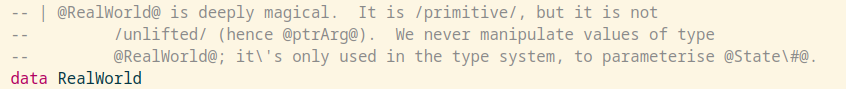
\includegraphics[width=0.9\textwidth]{figs/real_world}
            \end{center}
            \item Каждая программа меняет мир, меняйте мир к лучшему!
            \begin{itemize}
                \item \mintinline{haskell}|main :: IO () -- RealWorld -> ((), RealWorld)|
            \end{itemize}
            \item Эффект \mintinline{haskell}|IO| выполняется только когда он повлиял на результирующий \mintinline{haskell}|RealWorld|
            \begin{itemize}
                \item[$-$] \mintinline{haskell}|main = let p = print 42 in pure ()|
                \item[$+$] \mintinline{haskell}|main = let p = print 42 in p *> pure ()|
            \end{itemize}
            \item \mintinline{haskell}|RealWorld| --- интерфейс ко всему могуществу операционной системы
            \item[\eg] Мутабельная память, потоки, синхронизация\ldots
        \end{itemize}
    \end{frame}

    \begin{frame}[fragile]{Картинки}
        \vspace{-0.5em}
        \begin{center}
            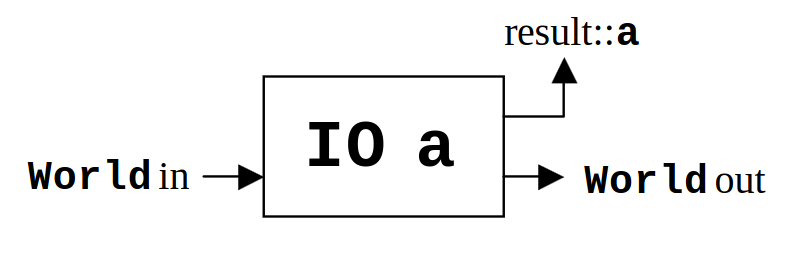
\includegraphics[width=0.4\textwidth]{figs/io1}

            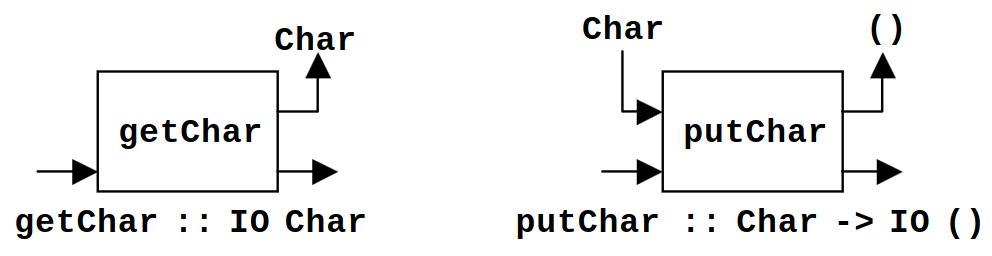
\includegraphics[width=0.5\textwidth]{figs/io2}

            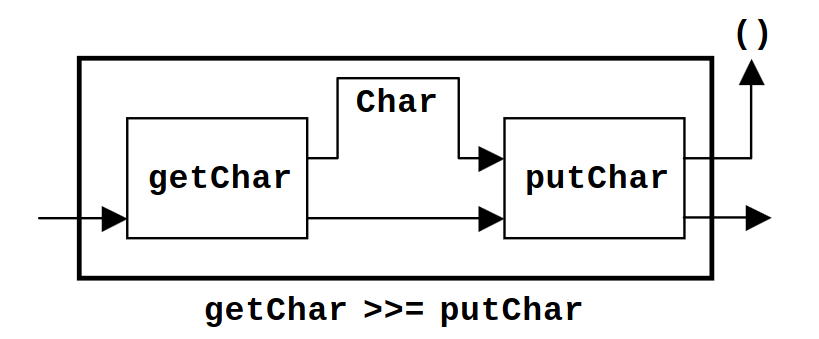
\includegraphics[width=0.5\textwidth]{figs/io3}
        \end{center}
    \end{frame}

    \begin{frame}[fragile]{Чистый язык и ``грязный'' runtime \popslide}
        \vspace{-0.5em}
        \begin{block}{Runtime}
            Два значения, нас интересует второе:
            \begin{itemize}
                \item[\defi] Промежуток времени, в который программа исполняется
                \item[\defi] Код, поставляемый вместе с ЯП, который существует в адресном пространстве программ на этом ЯП и помогает им исполняться
                \begin{itemize}
                    \item[\eg] garbage collector (GC), entry point --- код до \mintinline{haskell}|main|\ldots
                \end{itemize}
            \end{itemize}
        \end{block}
        \begin{itemize}
            \item Незапущенная программа на Haskell --- чистая функция, реальность --- персистентная структура данных
            \item Запуск программы передаёт управление entry point, которая конструирует RealWorld и передаёт написанному ``чистому'' \mintinline{haskell}|main|
            \item Haskell остаётся чистым языком программирования, это только runtime грязный!
        \end{itemize}
    \end{frame}

    \begin{frame}[fragile]{Контроль чистоты вычислений}
        \vspace{-0.5em}
        \begin{itemize}
            \item Из \mintinline{haskell}|IO| нельзя достать значение кроме как в bind
            \item Вычисление, один раз ставшее ``грязным'', ``заражает'' все зависящие вычисления
            \item Отслеживаем в \mintinline{haskell}|IO|, какие вычисления завязаны на кошмар реальности
            \item[\positive] Типы отделяют чистые вычисления от ``грязных''
            \item[\positive] Нужно максимизировать чистую часть программы, локализуя ``грязную''
            \item[\positive] На побочные эффекты распространяются алгебраические законы монад
        \end{itemize}
    \end{frame}

    \begin{frame}[fragile]{Минимизируем ``грязную'' часть программы\footnote{Картинка из книги Haskell in Depth Виталия Брагилевского.}}
        \vspace{-0.5em}
        \begin{center}
            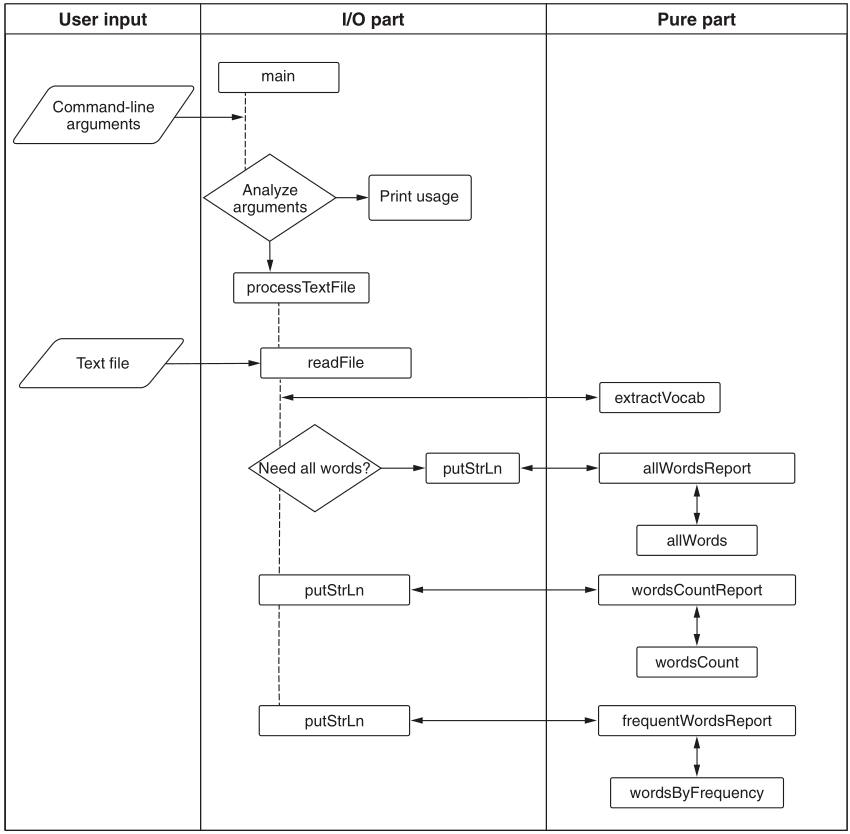
\includegraphics[height=0.8\textheight]{figs/pure}
        \end{center}
    \end{frame}

    \begin{frame}[fragile]{Hello world}
        \pause
        \vspace{-1em}
        \begin{columns}[onlytextwidth]
            \begin{column}[t]{0.3\textwidth}
            \end{column}\hfill%
            \begin{column}[t]{0.7\textwidth}
                \begin{minted}{haskell}
                main :: IO ()
                main = putStrLn "Hello world!"
                \end{minted}
            \end{column}
        \end{columns}
        \pause
        \begin{center}
            
\includegraphics[width=0.6\textwidth]{figs/hello_world}
        \end{center}
    \end{frame}

    \sectionplan{Материалы}

    \begin{frame}[fragile]{Что посмотреть в транспорте}
        \begin{itemize}
            \item \href{https://youtu.be/qgfCmQ-2tW0?si=9OBcKAlmGovWzSLp}{\color{blue} Keynote: Daniel Spiewak - The Case For Effect Systems}
            \item \href{https://youtu.be/M0Fe2SRTm5c?si=34lMmVWtRjPg9OYj}{\color{blue} John De Goes: One Monad to Rule Them All }
        \end{itemize}
    \end{frame}

    \begin{frame}[fragile]{Материалы}
        \begin{itemize}
            \item {\color{blue} \url{https://wiki.haskell.org/IO_inside}}
            \item \href{https://citeseerx.ist.psu.edu/document?repid=rep1&type=pdf&doi=2e6c9d76f9cb690dc18019fc894ba9572a8c2812}{\color{blue} Jones, S.P., 2001. Tackling the awkward squad: monadic input/output, concurrency, exceptions, and foreign-language calls in Haskell. NATO SCIENCE SERIES SUB SERIES III COMPUTER AND SYSTEMS SCIENCES, 180, pp.47-96.}
            \item {\color{blue}Marlow, Simon. "Parallel and concurrent programming in Haskell." \textit{Central European Functional Programming School}. Berlin, Heidelberg: Springer Berlin Heidelberg, 2011. 339-401.}
        \end{itemize}
    \end{frame}

\end{document}
